\section{Overview}

This supplementary material provides additional details and analyses complementing the main paper. It is organized as follows:

\begin{enumerate}

\item \textbf{Generation-based Comparison (Sec.~\ref{sec:gen_comp})}. 
We compare our method with a diffusion-based novel view generation approach, \textbf{SEVA}~\cite{zhou2025stable}, to highlight the differences between generation-based pipelines and our outpainting-based sparse-view reconstruction framework.

\item \textbf{Implementation Details (Sec.~\ref{sec:impl})}. 
We provide detailed implementation information for GaMO, including preprocessing, diffusion inference settings, mask generation, and integration with 3D Gaussian Splatting.

\item \textbf{Outpainting Comparison with Multi-View Diffusion Models (Sec.~\ref{sec:outpaint_comp})}. 
We evaluate different diffusion backbones for the outpainting stage and analyze their impact on reconstruction quality and geometric consistency.

\item \textbf{Iterative Mask Scheduling (Sec.~\ref{sec:ims})}. 
We present additional details and visualizations of the proposed iterative mask scheduling strategy and its effect on boundary coherence and generation stability.

\item \textbf{Additional Quantitative Comparisons (Sec.~\ref{sec:quant})}. 
We report extended quantitative evaluations across datasets and sparse-view settings (3, 6, and 9 views).

\item \textbf{Additional Qualitative Comparisons (Sec.~\ref{sec:qual})}. 
We provide additional visual comparisons illustrating reconstruction quality and scene completeness.

\item \textbf{Runtime Analysis (Sec.~\ref{sec:runtime})}. 
We analyze the computational efficiency of GaMO and compare runtime with existing diffusion-based reconstruction pipelines.

\item \textbf{Failure Cases (Sec.~\ref{sec:failure})}. 
We present representative failure cases and discuss limitations of the proposed approach.

\item \textbf{Baseline Implementation Details (Sec.~\ref{sec:baseline})}. 
We describe the implementation details of all baseline methods, including training configurations, initialization strategies, and evaluation protocols.

\item \textbf{Per-Scene Quantitative Results (Sec.~\ref{sec:per_scene})}. 
We report detailed PSNR, SSIM, and LPIPS results for every scene across Replica~\cite{straub2019replica}, ScanNet++~\cite{yeshwanth2023scannet++}, and Mip-NeRF 360~\cite{barron2023mipnerf360}.

\end{enumerate}

In addition, we provide an interactive HTML visualization (\texttt{main.html}) showing rendered videos along novel-view trajectories across scenes, enabling qualitative inspection of reconstruction quality beyond the input viewpoints.


\section{Generation-based Comparison}
\label{sec:gen_comp}

To further compare with approaches designed for direct novel view generation, we evaluate our method against the diffusion-based method SEVA~\cite{zhou2025stable}. As shown in Table~\ref{tab:seva_comparison}, our approach consistently outperformed SEVA across both datasets and view settings. In particular, our method achieved significantly higher PSNR and SSIM while reducing LPIPS, indicating more accurate reconstruction and better perceptual quality.

Qualitative results in Fig.~\ref{fig:ablation_1} further illustrated these differences. While SEVA produced visually plausible results, it often exhibited inaccurate pixel-level details and geometrically inconsistent structures. In contrast, our method preserved accurate details and more coherent scene geometry.

\vspace{-10pt}



\begin{figure}[ht]
    \centering
    \footnotesize
    \begin{minipage}[t]{0.48\textwidth}
        \vspace{0pt}
        \captionof{table}{\textbf{Comparison with the diffusion-based novel view generation method SEVA.} 
        We report PSNR$\uparrow$, SSIM$\uparrow$, and LPIPS$\downarrow$.}
        \label{tab:seva_comparison}
        \resizebox{\linewidth}{!}{
        \setlength{\tabcolsep}{4pt}
        \renewcommand{\arraystretch}{1.15}
        \begin{tabular}{l!{\vrule}ccc!{\vrule}ccc}
            \toprule
            & \multicolumn{3}{c!{\vrule}}{\textbf{Replica (3v)}}
            & \multicolumn{3}{c}{\textbf{ScanNet++ (3v)}} \\
            \cmidrule(lr){2-4}\cmidrule(lr){5-7}
            & PSNR & SSIM & LPIPS & PSNR & SSIM & LPIPS \\
            \midrule
            SEVA & 18.52 & 0.677 & 0.193 & 15.79 & 0.631 & 0.343 \\
            Ours & \textbf{25.40} & \textbf{0.864} & \textbf{0.117}
                 & \textbf{20.01} & \textbf{0.765} & \textbf{0.266} \\
            \midrule
            & \multicolumn{3}{c!{\vrule}}{\textbf{Replica (6v)}}
            & \multicolumn{3}{c}{\textbf{ScanNet++ (6v)}} \\
            \cmidrule(lr){2-4}\cmidrule(lr){5-7}
            & PSNR & SSIM & LPIPS & PSNR & SSIM & LPIPS \\
            \midrule
            SEVA & 18.64 & 0.691 & 0.206 & 16.93 & 0.640 & 0.276 \\
            Ours & \textbf{25.84} & \textbf{0.877} & \textbf{0.109}
                 & \textbf{23.41} & \textbf{0.835} & \textbf{0.181} \\
            \bottomrule
        \end{tabular}
        }
    \end{minipage}
    \hfill
    \begin{minipage}[t]{0.50\textwidth}
        \vspace{2mm}
        \centering
        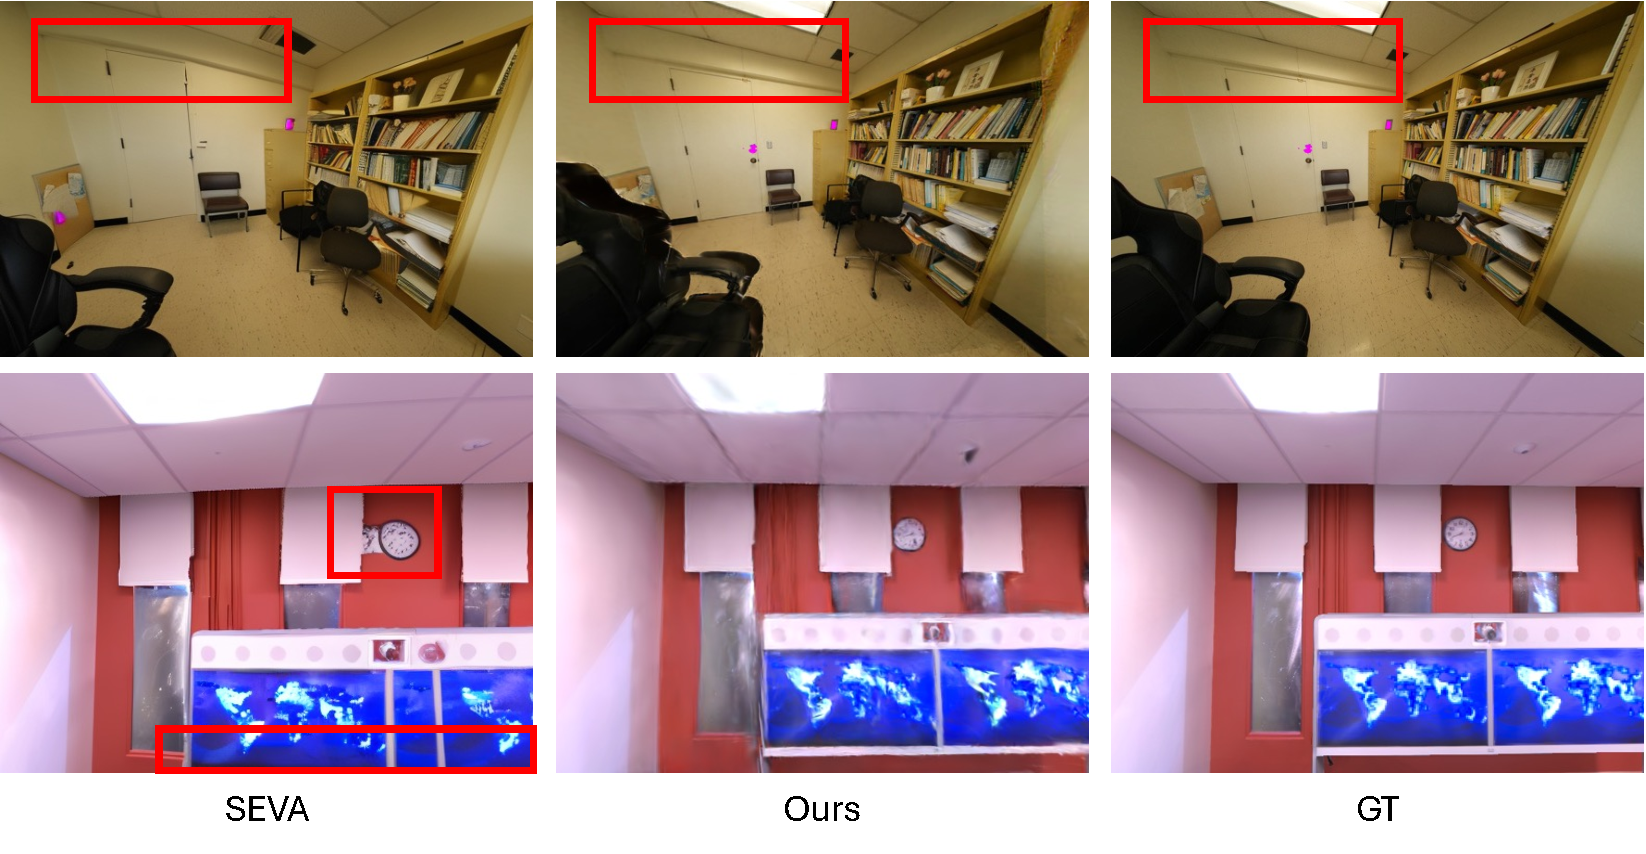
\includegraphics[width=\linewidth]{figures/SEVA.pdf}
        \vspace{-6mm}
        \caption{\textbf{Qualitative comparison with SEVA.} 
While SEVA produces visually plausible results, it often lacks pixel-level accuracy and geometric consistency.}
        \label{fig:ablation_1}
    \end{minipage}
\end{figure}


\vspace{-10pt}



\section{Implementation Details}
\label{sec:impl}

For coarse initialization, we train 3DGS for 10,000 iterations with $\lambda_s = 0.2$ and opacity threshold $\eta_{\text{mask}} = 0.6$. 

For outpainting, we use the multi-view diffusion model~\cite{cao2025mvgenmaster} with focal-length scaling $S_k \in [0.5, 0.7]$, adjusted per scene depending on scene scale. We use DDIM sampling~\cite{song2021denoising} with $T = 50$ steps, and perform latent blending at timesteps $t_1 = 0.7T$, $t_2 = 0.5T$, $t_3 = 0.3T$ with noise resampling $R = 3$. Input and outpainted views share the same resolution (differing only in FOV), with dimensions set as multiples of 64. Before refinement, we alpha-blend downscaled inputs at the center. 

For refinement, we optimize 3DGS for 3,000 iterations (3 views) or 7,000 iterations (6/9 views) with $\lambda_{\text{perc}} = 0.1$, alternating supervision between input and outpainted views. In addition, we make minor adjustments to several 3DGS refinement hyperparameters based on scene characteristics to ensure stable optimization. We will release all code, configurations, and scripts used in our experiments. All experiments are conducted on a single NVIDIA RTX 4090 GPU.

\section{Outpainting Comparison Using Multi-View Diffusion Models}
\label{sec:outpaint_comp}

\vspace{-10pt}
\begin{figure}[ht]
    \centering
    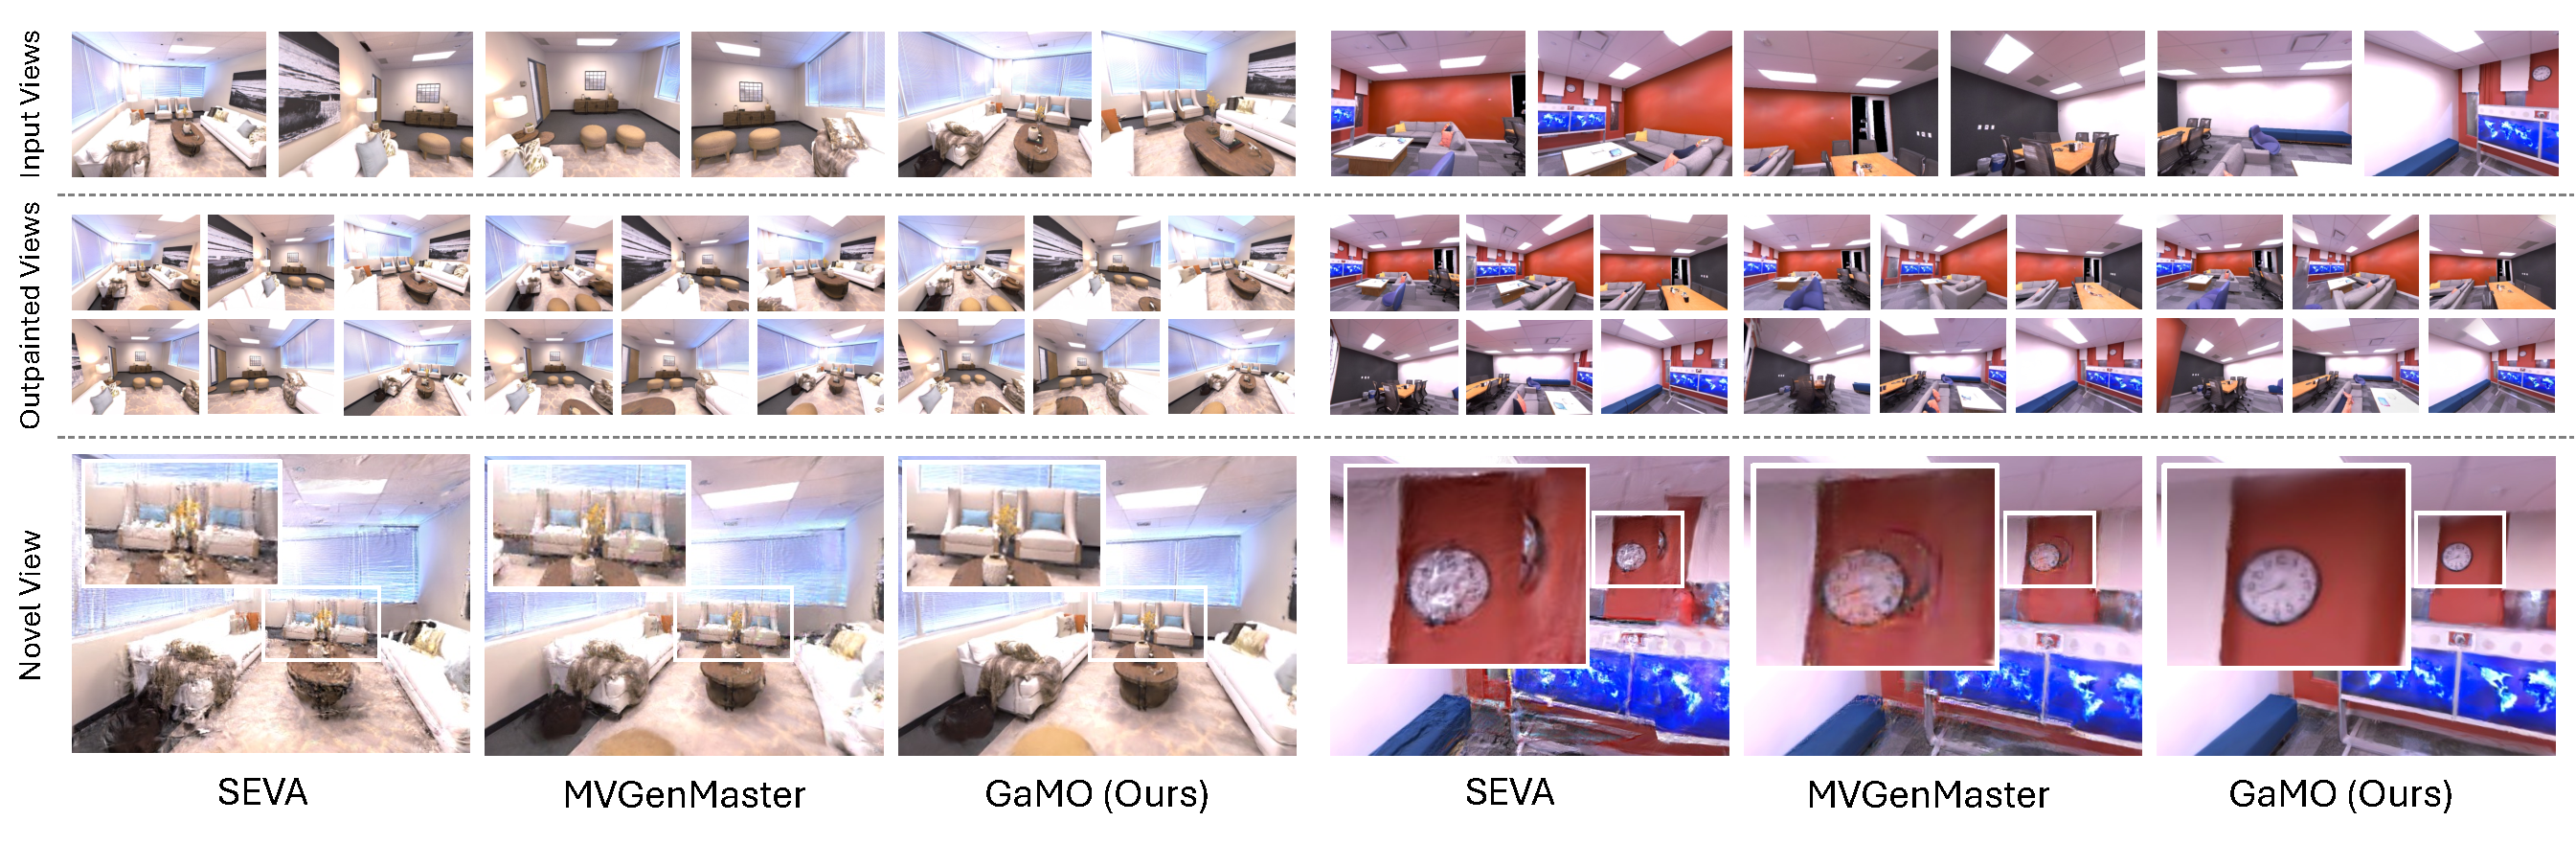
\includegraphics[width=\linewidth]{figures/sup_out.pdf}
    \vspace{-6mm}
    \caption{
        \textbf{Comparison of outpainting using adapted multi-view diffusion models.}
        Top: input views. 
        Middle: outpainted views generated by adapted SEVA~\cite{zhou2025stable}, MVGenMaster~\cite{cao2025mvgenmaster}, and our GaMO. 
        Bottom: novel views after 3DGS refinement using the generated outpainted views.
        Adapted multi-view diffusion models suffer from multi-view inconsistency, resulting in noisy reconstructions, while our method produces consistent outpainted views that improve reconstruction quality.
    }
    \label{fig:mv_diffusion_comparison}
\end{figure}


We compare our method against adapted multi-view diffusion models for outpainting. Specifically, we adapt SEVA~\cite{zhou2025stable} and MVGenMaster~\cite{cao2025mvgenmaster} 
by modifying the camera intrinsics to generate outpainted versions of the input views with 
extended FOV. These outpainted input views are then used to train 3DGS for improved novel 
view synthesis.

As shown in Fig.~\ref{fig:mv_diffusion_comparison}, SEVA produces highly noisy novel views after 3DGS refinement due to severe multi-view inconsistency caused by lack of geometric constraints. While MVGenMaster incorporates additional geometric mechanisms (e.g., multi-view conditioning), it still suffers from inconsistency issues that introduce artifacts in the refined reconstruction. In contrast, our GaMO effectively addresses the multi-view inconsistency problem, providing consistent outpainted views across multiple viewpoints that successfully refine 3DGS quality without introducing additional noise or artifacts. 



\begin{wrapfigure}{r}{0.45\textwidth}
    \vspace{-12mm}
    \centering
    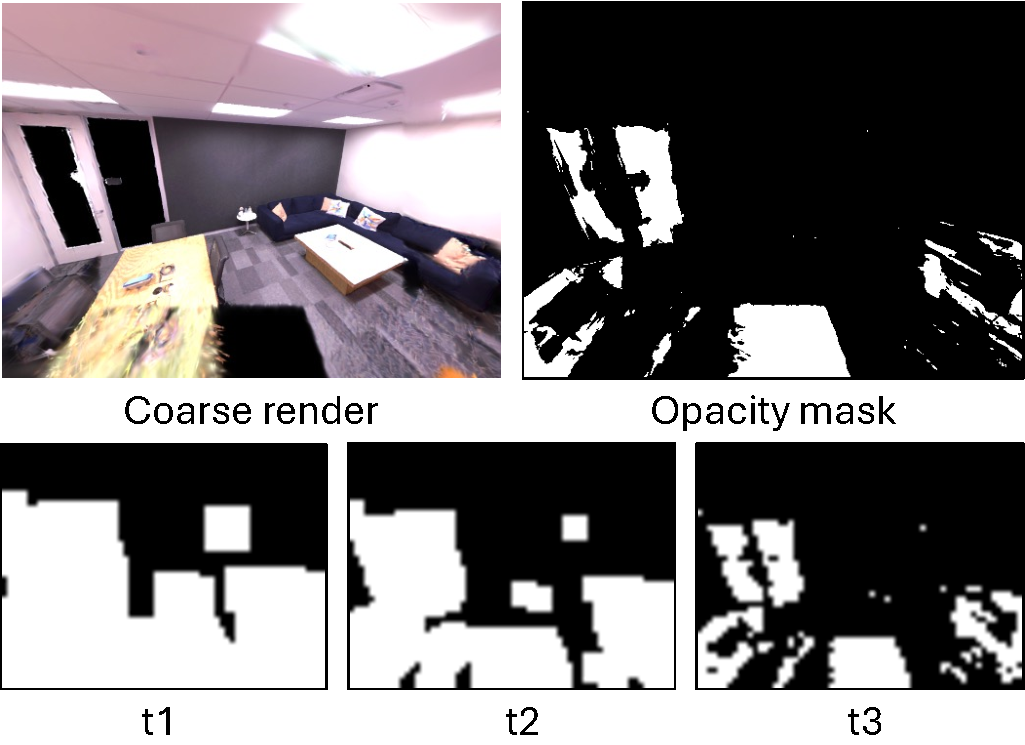
\includegraphics[width=\linewidth]{figures/IMS.pdf}
    \vspace{-8mm}
    \caption{
    \textbf{Iterative Mask Scheduling visualization.}
    Top: coarse render and opacity mask derived from the coarse 3D initialization.
    Bottom: progressive mask shrinking during denoising at timesteps $t = 35, 25, 15$, with 2, 1, and 0 dilation iterations, respectively.
    }
    \label{fig:ims_vis}
    \vspace{-12mm}
\end{wrapfigure}
\section{Iterative Mask Scheduling Implementation}
\label{sec:ims}


To maximize the utilization of coarse geometry during outpainting while preserving the generative diversity of the diffusion model, we introduce an \textbf{Iterative Mask Scheduling (IMS)} strategy. IMS dynamically adjusts the mask region throughout the denoising process, allowing the diffusion model to first freely hallucinate missing regions and later progressively align the generated content with the coarse 3D initialization.



\noindent\textbf{Design Rationale.} 
As demonstrated in the ablation studies in the main paper (Tab. 3), we found that applying mask latent blending at specific denoising steps yields significantly better results than continuous blending throughout the entire denoising process. Based on these findings, we strategically select three representative timesteps corresponding to the early, middle, and late stages of denoising to participate in the latent blending process. At each stage, we employ progressively shrinking mask sizes to control the degree of interference with the denoising process: larger masks in early stages allow more freedom for generation, while smaller masks in later stages enforce stronger alignment with coarse geometry.




\noindent\textbf{Implementation Details.}
As illustrated in Fig.~\ref{fig:ims_vis}, we generate three mask levels through morphological dilation:
\begin{equation}
\mathcal{M}_{\text{latent}}^{(k)} = \text{Dilate}(\mathcal{M}_{\text{base}}^{\downarrow}, \text{kernel}=5, \text{iterations}=\frac{k-15}{10}),
\end{equation}
where $\mathcal{M}_{\text{base}}^{\downarrow}$ denotes the downsampled base mask from the coarse geometry opacity map, aligned to the latent space resolution of $64 \times 48$ via adaptive max pooling. The $\text{Dilate}(\cdot)$ operation applies iterative max pooling with $5 \times 5$ kernel to expand the masked region. During the denoising process from $t = 50$ to $t = 0$, we apply $\mathcal{M}_{\text{latent}}^{(35)}$ at $t = 35$, $\mathcal{M}_{\text{latent}}^{(25)}$ at $t = 25$, and $\mathcal{M}_{\text{latent}}^{(15)}$ at $t = 15$, as visualized in Fig.~\ref{fig:ims_vis}. This staged approach balances generative freedom with geometric consistency, as validated by our ablation experiments.






\section{More Quantitative Comparison}
\label{sec:quant}
We provide additional quantitative results on Replica~\cite{straub2019replica} and ScanNet++~\cite{yeshwanth2023scannet++} datasets with varying numbers of input views (3, 6, and 9 views), as shown in Tab.~\ref{tab:replica_3_6_9} and Tab.~\ref{tab:scannetpp_3_6_9}. We focus our comparison on 3DGS~\cite{kerbl20233d} and GuidedVD-3DGS~\cite{zhong2025taming}, a competitive state-of-the-art diffusion-based method.

\noindent\textbf{Evaluation Protocol.}
For Replica, we follow the evaluation protocol from~\cite{zhong2025taming} for all three view settings. For ScanNet++, the 6-view setting follows~\cite{zhong2025taming}, while the 3-view and 9-view settings use manually selected views to maximize spatial coverage. All methods use DUSt3R~\cite{wang2024dust3r} for point cloud initialization.

\noindent\textbf{Results.}
Our method consistently outperforms baselines across most metrics and view settings. On Replica, we achieve the best SSIM and LPIPS scores across all view counts. On ScanNet++, we obtain superior performance across all metrics in all view settings. Notably, our method maintains competitive quality with GuidedVD-3DGS~\cite{zhong2025taming} while being significantly faster (approximately 6-9 minutes vs. 3+ hours).


\begin{table*}[h!]
\centering
\scriptsize
\setlength{\tabcolsep}{3pt}
\caption{\textbf{Quantitative comparison on Replica~\cite{straub2019replica} with 3, 6, and 9 input views.}}
\label{tab:replica_3_6_9}
\vspace{-3mm}
\begin{tabular}{l!{\vrule}ccc!{\vrule}ccc!{\vrule}ccc}
\toprule
\multirow{2}{*}{Method} &
\multicolumn{3}{c!{\vrule}}{Replica (3 views)} &
\multicolumn{3}{c!{\vrule}}{Replica (6 views)} &
\multicolumn{3}{c}{Replica (9 views)} \\
\cmidrule(lr){2-4} \cmidrule(lr){5-7} \cmidrule(lr){8-10}
& PSNR & SSIM & LPIPS & PSNR & SSIM & LPIPS & PSNR & SSIM & LPIPS \\
\midrule
3DGS~\cite{kerbl20233d}
    & 20.39 & 0.818 & 0.154
    & 24.41 & 0.862 & \cellcolor{orange!25}0.124
    & 26.09 & 0.890 & \cellcolor{orange!25}0.100 \\
GuidedVD-3DGS~\cite{zhong2025taming}
    & \cellcolor{red!25}25.26 & \cellcolor{orange!25}0.864 & \cellcolor{orange!25}0.138
    & \cellcolor{red!25}26.68 & \cellcolor{orange!25}0.880 & 0.133
    & \cellcolor{red!25}28.08 & \cellcolor{orange!25}0.901 & 0.108 \\
Ours
    & \cellcolor{orange!25} 24.40 & \cellcolor{red!25}0.865 & \cellcolor{red!25}0.117
    & \cellcolor{orange!25}26.40 & \cellcolor{red!25}0.882 & \cellcolor{red!25}0.104
    & \cellcolor{orange!25} 27.58 & \cellcolor{red!25} 0.902 & \cellcolor{red!25} 0.096 \\
\bottomrule
\end{tabular}
\end{table*}

\begin{table*}[h!]
\centering
\scriptsize
\setlength{\tabcolsep}{3pt}
\caption{\textbf{Quantitative comparison on ScanNet++~\cite{yeshwanth2023scannet++} with 3, 6, and 9 input views.}}
\label{tab:scannetpp_3_6_9}
\vspace{-3mm}
\begin{tabular}{l!{\vrule}ccc!{\vrule}ccc!{\vrule}ccc}
\toprule
\multirow{2}{*}{Method} &
\multicolumn{3}{c!{\vrule}}{ScanNet++ (3 views)} &
\multicolumn{3}{c!{\vrule}}{ScanNet++ (6 views)} &
\multicolumn{3}{c}{ScanNet++ (9 views)} \\
\cmidrule(lr){2-4} \cmidrule(lr){5-7} \cmidrule(lr){8-10}
& PSNR & SSIM & LPIPS & PSNR & SSIM & LPIPS & PSNR & SSIM & LPIPS \\
\midrule
3DGS~\cite{kerbl20233d}
    & 16.60 & 0.710 & 0.313
    & 21.71 & 0.808 & \cellcolor{orange!25}0.186
    & 24.55 & \cellcolor{orange!25}0.845 & \cellcolor{orange!25}0.155 \\
GuidedVD-3DGS~\cite{zhong2025taming}
    & \cellcolor{orange!25}19.93 & \cellcolor{orange!25}0.759 & \cellcolor{orange!25}0.297
    & \cellcolor{orange!25}22.98 & \cellcolor{orange!25}0.815 & 0.204
    & \cellcolor{orange!25}24.65 & 0.843 & 0.159 \\
Ours
    & \cellcolor{red!25}20.00 & \cellcolor{red!25}0.765 & \cellcolor{red!25}0.268
    & \cellcolor{red!25}23.41 & \cellcolor{red!25}0.835 & \cellcolor{red!25}0.181
    & \cellcolor{red!25}25.17 & \cellcolor{red!25}0.860 & \cellcolor{red!25}0.152 \\
\bottomrule
\end{tabular}
\end{table*}





\section{More Qualitative Comparison}
\label{sec:qual}

We provide additional qualitative results across 3-, 6-, and 9-view settings on Replica~\cite{straub2019replica} and ScanNet++~\cite{yeshwanth2023scannet++} datasets, as shown in Fig.~\ref{fig:comparison}. We compare against 3DGS~\cite{kerbl20233d}, FSGS~\cite{zhu2024fsgs}, InstantSplat~\cite{fan2024instantsplat}, DiFix3D~\cite{wu2025difix3d+}, GenFusion~\cite{wu2025genfusion}, and GuidedVD-3DGS~\cite{zhong2025taming} using the same baseline configurations as described in the main paper.

As illustrated in Fig~\ref{fig:comparison}, even with extremely sparse inputs (3 views), our method produces reasonable content and geometry while maintaining consistency. Compared to baselines, our approach demonstrates better scene coverage with fewer missing regions (black holes), improved geometric consistency with reduced ghosting artifacts, and overall higher visual quality. These improvements are particularly evident in challenging regions highlighted by white boxes.






\begin{figure*}[h!]
    \centering
    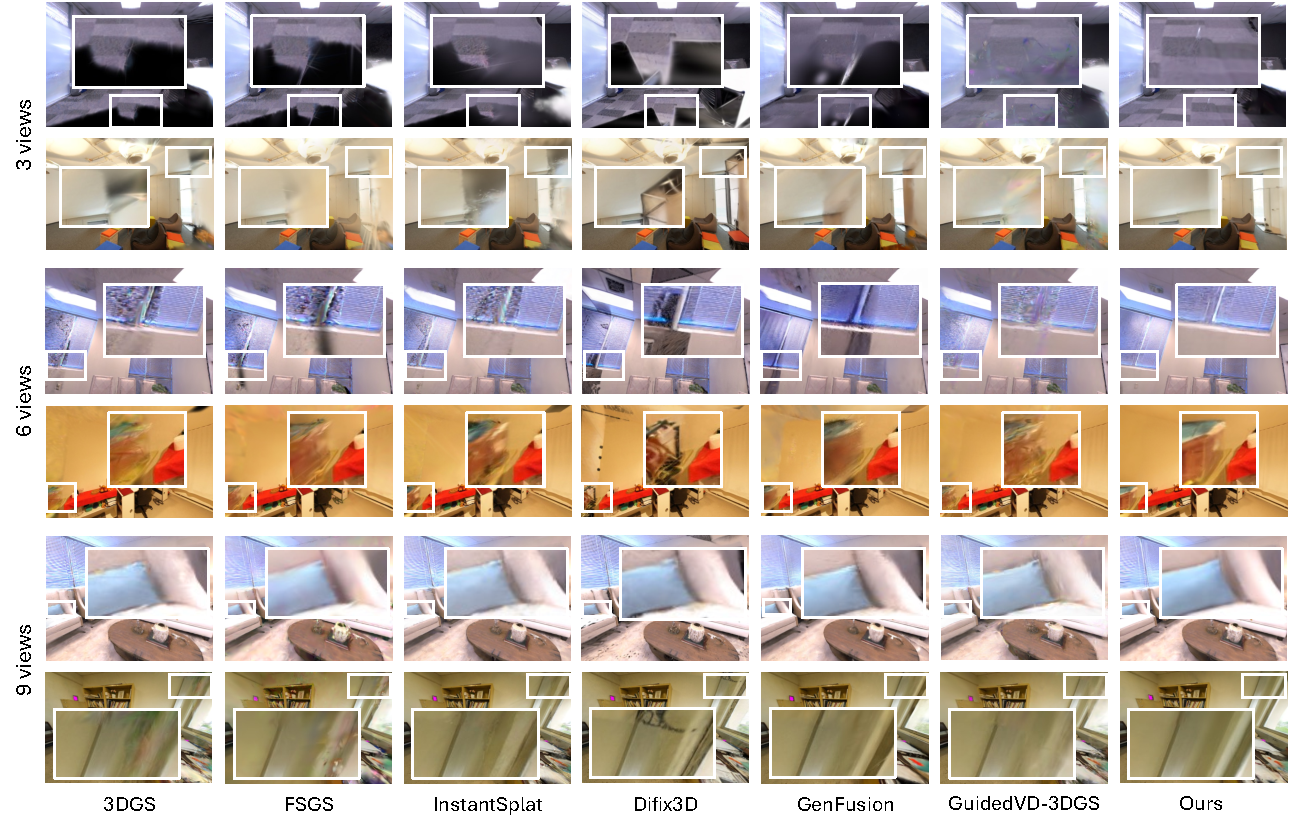
\includegraphics[width=\linewidth]{figures/Qualitative.pdf}
    \vspace{-6mm}
    \caption{
        \textbf{Qualitative comparison on Replica~\cite{straub2019replica} and ScanNet++~\cite{yeshwanth2023scannet++} with 3, 6, and 9 sparse views.}
        Our method produces better coverage, geometric consistency, and fewer artifacts compared to baselines.
        White boxes highlight challenging regions. Best viewed zoomed in.
    }
    \label{fig:comparison}
\end{figure*}




\section{Runtime Analysis}
\label{sec:runtime}


\begin{wrapfigure}{r}{0.45\textwidth}
    \vspace{-25pt}
    \centering
    \footnotesize
    \setlength{\abovecaptionskip}{0pt}
    \setlength{\belowcaptionskip}{2pt}
    \captionof{table}{\textbf{Runtime breakdown of our method on (RTX 4090).}}
    \label{tab:runtime}
    \resizebox{\linewidth}{!}{
    \setlength{\tabcolsep}{4pt}
    \renewcommand{\arraystretch}{1.15}
    \begin{tabular}{lcc}
        \toprule
        Stage & Time (s) & Time (min) \\
        \midrule
        Coarse 3DGS init.\ \& render & 118 & 1.97 \\
        Multi-view outpainting & 93 & 1.55 \\
        3DGS refine (train + render) & 280 & 4.67 \\
        \midrule
        Total & 491 & 8.18 \\
        \bottomrule
    \end{tabular}
    }
    \vspace{4pt}
    \captionof{table}{\textbf{End-to-end runtime comparison (RTX A6000).}}
    \label{tab:runtime_a6000}
    \resizebox{\linewidth}{!}{
    \setlength{\tabcolsep}{4pt}
    \renewcommand{\arraystretch}{1.15}
    \begin{tabular}{lc}
        \toprule
        Method & Total Time \\
        \midrule
        GuidedVD-3DGS~\cite{zhong2025taming} & $\sim$3h 20min \\
        Ours & \textbf{9min 54s} \\
        \bottomrule
    \end{tabular}
    }
    \vspace{-30pt}
\end{wrapfigure}

We report the end-to-end runtime of our pipeline on a representative indoor scene (Replica\_6, \textit{office\_2}) with 6 input views at $512 \times 384$ resolution, evaluated on a single NVIDIA RTX 4090 GPU. The pipeline consists of three main stages: coarse 3DGS reconstruction and rendering, multi-view diffusion outpainting, and the final 3DGS refinement stage that incorporates DUSt3R point cloud initialization and refined 3DGS training.

Since GuidedVD-3DGS requires significantly larger GPU memory, it is evaluated on an NVIDIA RTX A6000 GPU. For a fair comparison, we additionally report the runtime of our method on the same hardware. On the Replica \textit{office\_2} scene, our pipeline takes \textbf{9 min 54 s}, while GuidedVD-3DGS requires approximately \textbf{3 hours 20 minutes}. This demonstrates that our method achieves substantially faster reconstruction while maintaining competitive reconstruction quality.



\section{Failure Cases}
\label{sec:failure}
While our method demonstrates strong performance across a wide range of scenarios, it remains limited in scenes containing severe occlusions. This limitation is inherent to all methods that generate novel views for 3D reconstruction; current multi-view diffusion models face the same challenge, as even densely sampled novel viewpoints struggle to reconstruct regions that are severely occluded by obstacles. As shown in Fig.~\ref{fig:failure_cases}, such heavily occluded areas remain challenging for both geometry-aware outpainting and multi-view diffusion methods.

\noindent\textbf{Potential Solutions.}
A promising direction to address viewpoint-specific occlusions is to generate outpainted views from alternative camera perspectives with geometry-aware mechanisms, such as bird's-eye or top-down views with a larger FOV. By generating content from drastically different viewing angles, these views could potentially observe regions that are occluded from the original camera poses, thereby providing complementary supervision for the occluded areas.

\begin{figure}[t]
\centering
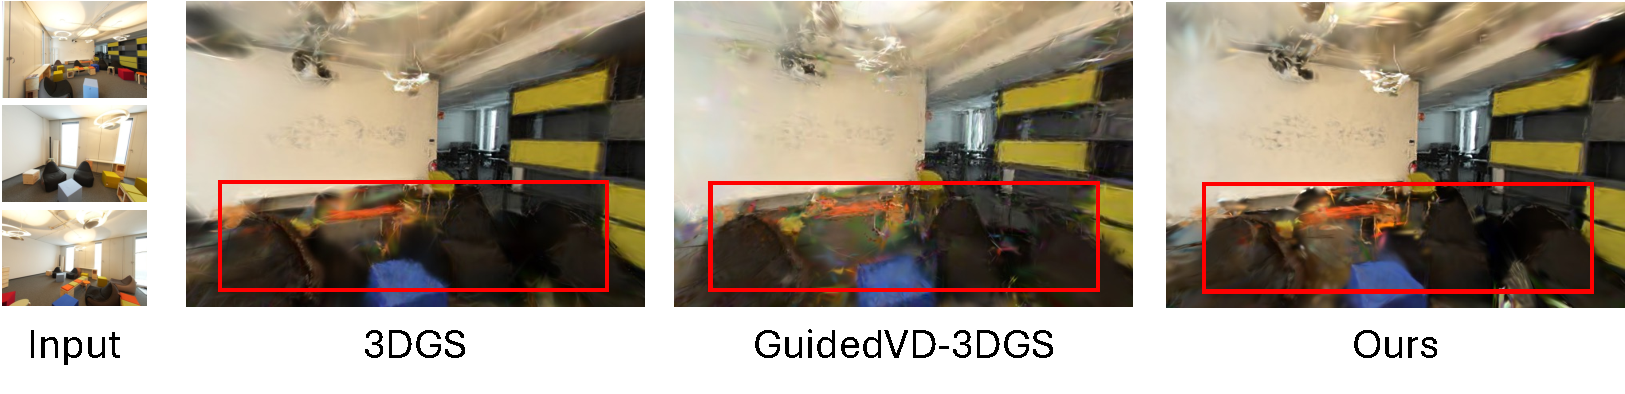
\includegraphics[width=\linewidth]{figures/Failure.pdf}
    \vspace{-6mm}
\caption{
\textbf{Failure cases in heavily occluded regions.}
Due to severe occlusions in the scene, certain regions are never observed across all input views. Both outpainting (ours) and novel view generation 
methods struggle to reconstruct these completely unobserved areas. Red boxes highlight the occluded regions where reconstruction fails.
}
\label{fig:failure_cases}
\end{figure}
\section{Baseline Implementation Details}
\label{sec:baseline}

In this section, we describe the implementation details of all baseline methods used in our experiments. Unless otherwise stated, we follow the official implementations and recommended settings provided by the authors. For most methods, the input camera poses are provided and the reconstruction is initialized using point clouds estimated by DUSt3R~\cite{wang2024dust3r}. InstantSplat follows its original pipeline and uses MASt3R~\cite{duisterhof2025mastrsfm} for initialization. Method-specific differences (e.g., initialization strategies) are described in the corresponding subsections.

%We provide additional qualitative results across 3-, 6-, and 9-view settings on Replica~\cite{straub2019replica} and ScanNet++~\cite{yeshwanth2023scannet++} datasets, as shown in Fig.~\ref{fig:comparison}. We compare against 3DGS~\cite{kerbl20233d}, FSGS~\cite{zhu2024fsgs}, InstantSplat~\cite{fan2024instantsplat}, DiFix3D~\cite{wu2025difix3d+}, GenFusion~\cite{wu2025genfusion}, and GuidedVD-3DGS~\cite{zhong2025taming} using the same baseline configurations as described in the main paper.

\paragraph{3DGS~\cite{kerbl20233d}.}
We use the vanilla 3D Gaussian Splatting implementation~\cite{kerbl20233d} with its default training settings. 
The Gaussian primitives are initialized using the DUSt3R point cloud described above, and the input camera poses are kept fixed during optimization.

\paragraph{FSGS~\cite{zhu2024fsgs}.}
For FSGS, we follow the official implementation and training configuration provided by the authors~\cite{zhu2024fsgs}. In particular, we adopt the version that incorporates the depth supervision term, as suggested in the original implementation. All other training parameters remain consistent with the default configuration.

\paragraph{InstantSplat~\cite{fan2024instantsplat}.}
InstantSplat is implemented using the official codebase~\cite{fan2024instantsplat} with its default settings. The Gaussian initialization is obtained from point clouds reconstructed using MASt3R~\cite{duisterhof2025mastrsfm}, following the standard pipeline described in the original work.

\paragraph{Difix3D+~\cite{wu2025difix3d+}.}
The Difix3D framework contains multiple variants. In the original implementation, \textit{DiFix3D} and \textit{DiFix3D+} correspond to different variants within the same framework~\cite{wu2025difix3d+}, differing in whether a time neural enhancer is used during inference. In our experiments, we adopt the version without the time neural enhancer to maintain consistency with the base reconstruction pipeline.

\paragraph{GenFusion~\cite{wu2025genfusion}.}
GenFusion is evaluated using the official implementation and recommended hyperparameters~\cite{wu2025genfusion}. We follow the standard training and inference pipeline without modifying any of the default settings.

\paragraph{GuidedVD-3DGS~\cite{zhong2025taming}.}
GuidedVD-3DGS is implemented using the official codebase~\cite{zhong2025taming}. However, the results reported in the original paper use a different rendering resolution compared to our evaluation protocol. This difference leads to minor numerical discrepancies between the reported numbers in the paper and those reproduced in our environment. For transparency and fair comparison, we report both the original results from the paper and the results reproduced under our experimental settings.

\section{Per-Scene Quantitative Results}
\label{sec:per_scene}

We provide detailed per-scene quantitative results for every method across all datasets and view settings. Tab.~\ref{tab:scannet_replica_3views_per_scene} reports results on ScanNet++ and Replica with 3 input views, Tab.~\ref{tab:scannet_replica_6views_per_scene} with 6 input views, and Tab.~\ref{tab:mipnerf360_per_scene} reports results on Mip-NeRF360 with 6 and 9 input views. Each entry reports PSNR, SSIM, and LPIPS from top to bottom. Our method achieves consistently strong performance across scenes and datasets, ranking first or second in the majority of per-scene metrics while maintaining competitive results throughout, all while being \textbf{20$\times$ faster} than the strongest competing method.


\begin{table}[H]
\centering
\tiny
\setlength{\tabcolsep}{2pt}
\renewcommand{\arraystretch}{1.25}
\caption{\textbf{Per-scene quantitative results on ScanNet++ and Replica (3 views).}
Each entry reports PSNR$\uparrow$, SSIM$\uparrow$, and LPIPS$\downarrow$ from top to bottom.}
\vspace{-4pt}
\label{tab:scannet_replica_3views_per_scene}

\begin{tabular}{l!{\vrule}ccccc!{\vrule}ccccccc}
\toprule
& \multicolumn{5}{c!{\vrule}}{\textsc{ScanNet++ (3 Views)}}
& \multicolumn{7}{c}{\textsc{Replica (3 Views)}} \\
\midrule
Method
& 8a20 & 94ee & 7831 & a29c & avg
& office\_2 & office\_3 & office\_4 & room\_0 & room\_1 & room\_2 & avg \\
\midrule
3DGS
& \makecell[c]{15.63\\0.640\\0.340}
& \makecell[c]{16.61\\0.747\\0.283}
& \makecell[c]{19.08\\0.724\\0.311}
& \makecell[c]{14.68\\0.673\\0.345}
& \makecell[c]{16.50\\0.696\\0.320}
& \makecell[c]{18.87\\0.853\\0.147}
& \makecell[c]{22.51\\0.870\\0.104}
& \makecell[c]{20.96\\0.852\\0.131}
& \makecell[c]{20.96\\0.852\\0.131}
& \makecell[c]{22.14\\0.829\\0.129}
& \makecell[c]{19.34\\0.757\\0.223}
& \makecell[c]{20.39\\0.818\\0.154} \\
\midrule
FSGS
& \makecell[c]{18.09\\0.689\\0.299}
& \makecell[c]{15.97\\0.718\\0.355}
& \makecell[c]{17.44\\0.666\\0.412}
& \makecell[c]{14.82\\0.688\\0.369}
& \makecell[c]{16.58\\0.690\\0.359}
& \makecell[c]{21.07\\0.872\\0.177}
& \makecell[c]{22.31\\0.864\\0.117}
& \makecell[c]{20.24\\0.846\\0.140}
& \makecell[c]{18.40\\0.719\\0.213}
& \makecell[c]{21.81\\0.801\\0.167}
& \makecell[c]{21.20\\0.789\\0.220}
& \makecell[c]{20.84\\0.815\\0.172} \\
\midrule
InstantSplat
& \makecell[c]{17.27\\0.733\\0.232}
& \makecell[c]{17.42\\0.754\\0.311}
& \makecell[c]{17.79\\0.694\\0.399}
& \makecell[c]{14.38\\0.698\\0.317}
& \makecell[c]{16.72\\0.720\\0.315}
& \makecell[c]{19.78\\0.862\\0.124}
& \makecell[c]{22.97\\0.879\\0.096}
& \makecell[c]{22.43\\0.872\\0.103}
& \makecell[c]{18.05\\0.729\\0.177}
& \makecell[c]{22.62\\0.822\\0.130}
& \makecell[c]{18.05\\0.726\\0.219}
& \makecell[c]{20.65\\0.815\\0.142} \\
\midrule
Difix3D+
& \makecell[c]{16.05\\0.656\\0.297}
& \makecell[c]{16.05\\0.692\\0.364}
& \makecell[c]{16.38\\0.650\\0.355}
& \makecell[c]{14.09\\0.636\\0.366}
& \makecell[c]{15.64\\0.659\\0.346}
& \makecell[c]{19.58\\0.834\\0.203}
& \makecell[c]{20.77\\0.838\\0.145}
& \makecell[c]{20.65\\0.836\\0.138}
& \makecell[c]{17.89\\0.712\\0.232}
& \makecell[c]{18.79\\0.737\\0.201}
& \makecell[c]{19.14\\0.742\\0.245}
& \makecell[c]{19.47\\0.783\\0.194} \\
\midrule
GenFusion
& \makecell[c]{20.58\\0.747\\0.356}
& \makecell[c]{16.63\\0.725\\0.344}
& \makecell[c]{17.46\\0.693\\0.376}
& \makecell[c]{17.22\\0.734\\0.340}
& \makecell[c]{17.97\\0.725\\0.354}
& \makecell[c]{22.43\\0.882\\0.165}
& \makecell[c]{23.53\\0.871\\0.138}
& \makecell[c]{23.46\\0.861\\0.156}
& \makecell[c]{19.40\\0.745\\0.215}
& \makecell[c]{24.18\\0.835\\0.142}
& \makecell[c]{21.02\\0.803\\0.216}
& \makecell[c]{22.34\\0.833\\0.172} \\
\midrule
GuidedVD-3DGS
& \makecell[c]{17.32\\0.642\\0.342}
& \makecell[c]{\textbf{19.04}\\0.756\\0.316}
& \makecell[c]{19.23\\0.716\\0.359}
& \makecell[c]{19.70\\0.764\\0.306}
& \makecell[c]{18.82\\0.720\\0.328}
& \makecell[c]{25.07\\0.905\\0.114}
& \makecell[c]{\textbf{26.80}\\0.910\\0.097}
& \makecell[c]{\textbf{25.63}\\\textbf{0.898}\\0.109}
& \makecell[c]{\textbf{24.14}\\\textbf{0.791}\\0.171}
& \makecell[c]{\textbf{26.84}\\\textbf{0.854}\\0.126}
& \makecell[c]{\textbf{23.08}\\0.825\\0.208}
& \makecell[c]{\textbf{25.26}\\0.864\\0.138} \\
\midrule
Ours
& \makecell[c]{\textbf{20.77}\\\textbf{0.753}\\\textbf{0.225}}
& \makecell[c]{18.81\\\textbf{0.770}\\\textbf{0.273}}
& \makecell[c]{\textbf{20.35}\\\textbf{0.748}\\\textbf{0.299}}
& \makecell[c]{\textbf{20.31}\\\textbf{0.766}\\\textbf{0.263}}
& \makecell[c]{\textbf{20.06}\\\textbf{0.759}\\\textbf{0.265}}
& \makecell[c]{\textbf{25.13}\\\textbf{0.913}\\\textbf{0.088}}
& \makecell[c]{25.68\\\textbf{0.911}\\\textbf{0.075}}
& \makecell[c]{24.57\\0.897\\\textbf{0.095}}
& \makecell[c]{23.71\\0.789\\\textbf{0.150}}
& \makecell[c]{25.17\\0.851\\\textbf{0.114}}
& \makecell[c]{22.14\\\textbf{0.827}\\\textbf{0.179}}
& \makecell[c]{24.40\\\textbf{0.865}\\\textbf{0.117}} \\
\bottomrule
\end{tabular}
\end{table}



\begin{table}[t]
\centering
\tiny
\setlength{\tabcolsep}{2pt}
\renewcommand{\arraystretch}{1.25}

\caption{\textbf{Per-scene quantitative results on ScanNet++ and Replica (6views).}
Each entry reports PSNR$\uparrow$, SSIM$\uparrow$, and LPIPS$\downarrow$ from top to bottom.}
\vspace{-4pt}

\label{tab:scannet_replica_6views_per_scene}

\begin{tabular}{l!{\vrule}ccccc!{\vrule}ccccccc}
\toprule

& \multicolumn{5}{c!{\vrule}}{\textsc{ScanNet++ (6 Views)}} 
& \multicolumn{7}{c}{\textsc{Replica (6 Views)}} \\

\midrule

Method
& 8a20 
& 94ee 
& 7831 
& a29c 
& avg 
& office\_2 
& office\_3 
& office\_4 
& room\_0 
& room\_1 
& room\_2 
& avg \\

\midrule

3DGS
& \makecell[c]{24.33\\0.868\\0.109}
& \makecell[c]{20.22\\0.819\\0.200}
& \makecell[c]{21.41\\0.765\\0.262}
& \makecell[c]{20.87\\0.821\\0.169}
& \makecell[c]{21.71\\0.818\\0.186}
& \makecell[c]{27.40\\0.922\\0.070}
& \makecell[c]{25.05\\0.889\\0.101}
& \makecell[c]{23.66\\0.866\\0.135}
& \makecell[c]{21.92\\0.794\\0.142}
& \makecell[c]{24.03\\0.846\\0.140}
& \makecell[c]{24.38\\0.854\\0.156}
& \makecell[c]{24.74\\0.862\\0.124} \\

\midrule

FSGS
& \makecell[c]{23.56\\0.831\\0.234}
& \makecell[c]{20.72\\0.755\\0.402}
& \makecell[c]{20.86\\0.806\\0.309}
& \makecell[c]{21.60\\0.812\\0.246}
& \makecell[c]{21.69\\0.801\\0.298}
& \makecell[c]{25.99\\0.903\\0.092}
& \makecell[c]{24.24\\0.877\\0.114}
& \makecell[c]{23.51\\0.866\\0.148}
& \makecell[c]{21.65\\0.772\\0.171}
& \makecell[c]{22.89\\0.820\\0.171}
& \makecell[c]{23.18\\0.836\\0.175}
& \makecell[c]{23.91\\0.846\\0.145} \\

\midrule

InstantSplat
& \makecell[c]{22.84\\0.844\\0.121}
& \makecell[c]{20.27\\0.815\\0.209}
& \makecell[c]{21.16\\0.761\\0.275}
& \makecell[c]{20.50\\0.822\\0.165}
& \makecell[c]{21.19\\0.811\\0.193}
& \makecell[c]{26.62\\0.913\\0.071}
& \makecell[c]{20.04\\0.850\\0.187}
& \makecell[c]{22.72\\0.864\\0.150}
& \makecell[c]{21.35\\0.782\\0.138}
& \makecell[c]{23.65\\0.835\\0.142}
& \makecell[c]{24.14\\0.850\\0.150}
& \makecell[c]{23.09\\0.849\\0.140} \\

\midrule

Difix3D+
& \makecell[c]{23.86\\0.811\\0.175}
& \makecell[c]{19.42\\0.765\\0.269}
& \makecell[c]{18.86\\0.695\\0.312}
& \makecell[c]{20.34\\0.784\\0.219}
& \makecell[c]{20.62\\0.764\\0.244}
& \makecell[c]{23.40\\0.862\\0.160}
& \makecell[c]{21.70\\0.845\\0.149}
& \makecell[c]{22.79\\0.831\\0.176}
& \makecell[c]{20.42\\0.747\\0.204}
& \makecell[c]{21.22\\0.776\\0.219}
& \makecell[c]{21.62\\0.800\\0.218}
& \makecell[c]{21.86\\0.810\\0.188} \\

\midrule

GenFusion
& \makecell[c]{24.69\\0.860\\0.127}
& \makecell[c]{21.01\\0.818\\0.211}
& \makecell[c]{20.21\\0.750\\0.312}
& \makecell[c]{21.91\\0.805\\0.221}
& \makecell[c]{21.96\\0.808\\0.218}
& \makecell[c]{25.82\\0.909\\0.085}
& \makecell[c]{23.42\\0.869\\0.127}
& \makecell[c]{24.91\\0.878\\0.139}
& \makecell[c]{23.57\\0.808\\0.149}
& \makecell[c]{23.04\\0.830\\0.165}
& \makecell[c]{23.14\\0.837\\0.187}
& \makecell[c]{23.98\\0.855\\0.142} \\

\midrule

GuidedVD-3DGS$^\dagger$
& \makecell[c]{\textcolor{gray}{25.10}\\\textcolor{gray}{0.882}\\\textcolor{gray}{0.118}}
& \makecell[c]{\textcolor{gray}{23.10}\\\textcolor{gray}{0.860}\\\textcolor{gray}{0.201}}
& \makecell[c]{\textcolor{gray}{22.16}\\\textcolor{gray}{0.803}\\\textcolor{gray}{0.269}}
& \makecell[c]{\textcolor{gray}{25.21}\\\textcolor{gray}{0.857}\\\textcolor{gray}{0.157}}
& \makecell[c]{\textcolor{gray}{23.89}\\\textcolor{gray}{0.850}\\\textcolor{gray}{0.182}}
& \makecell[c]{\textcolor{gray}{27.46}\\\textcolor{gray}{0.916}\\\textcolor{gray}{0.083}}
& \makecell[c]{\textcolor{gray}{26.81}\\\textcolor{gray}{0.902}\\\textcolor{gray}{0.099}}
& \makecell[c]{\textcolor{gray}{27.43}\\\textcolor{gray}{0.897}\\\textcolor{gray}{0.122}}
& \makecell[c]{\textcolor{gray}{24.85}\\\textcolor{gray}{0.796}\\\textcolor{gray}{0.145}}
& \makecell[c]{\textcolor{gray}{26.00}\\\textcolor{gray}{0.851}\\\textcolor{gray}{0.142}}
& \makecell[c]{\textcolor{gray}{25.53}\\\textcolor{gray}{0.872}\\\textcolor{gray}{0.142}}
& \makecell[c]{\textcolor{gray}{26.35}\\\textcolor{gray}{0.872}\\\textcolor{gray}{0.122}} \\

\midrule

GuidedVD-3DGS$^\ddagger$
& \makecell[c]{24.18\\0.844\\0.143}
& \makecell[c]{22.11\\0.824\\0.219}
& \makecell[c]{\textbf{21.84}\\0.768\\0.283}
& \makecell[c]{23.79\\0.824\\0.172}
& \makecell[c]{22.98\\0.815\\0.204}
& \makecell[c]{\textbf{28.04}\\0.925\\0.087}
& \makecell[c]{\textbf{26.46}\\\textbf{0.901}\\0.112}
& \makecell[c]{\textbf{27.63}\\0.900\\0.130}
& \makecell[c]{25.55\\0.823\\0.143}
& \makecell[c]{\textbf{26.18}\\\textbf{0.858}\\0.157}
& \makecell[c]{\textbf{26.24}\\0.871\\0.167}
& \makecell[c]{\textbf{26.68}\\0.880\\0.133} \\

\midrule

Ours
& \makecell[c]{\textbf{24.98}\\\textbf{0.877}\\\textbf{0.104}}
& \makecell[c]{\textbf{22.38}\\\textbf{0.840}\\\textbf{0.186}}
& \makecell[c]{21.56\\\textbf{0.783}\\\textbf{0.269}}
& \makecell[c]{\textbf{24.70}\\\textbf{0.841}\\\textbf{0.164}}
& \makecell[c]{\textbf{23.41}\\\textbf{0.835}\\\textbf{0.181}}
& \makecell[c]{28.18\\\textbf{0.927}\\\textbf{0.062}}
& \makecell[c]{26.23\\0.900\\\textbf{0.087}}
& \makecell[c]{26.85\\\textbf{0.900}\\\textbf{0.104}}
& \makecell[c]{\textbf{25.65}\\\textbf{0.831}\\\textbf{0.117}}
& \makecell[c]{25.47\\0.857\\\textbf{0.127}}
& \makecell[c]{26.00\\\textbf{0.878}\\\textbf{0.128}}
& \makecell[c]{26.40\\\textbf{0.882}\\\textbf{0.104}} \\

\bottomrule
\end{tabular}

\vspace{-4pt}
\begin{flushleft}
\scriptsize $^\dagger$ Reported in paper, $^\ddagger$ Our reproduction.
\end{flushleft}

\end{table}



\begin{table}[H]
\centering
\tiny
\setlength{\tabcolsep}{1.4pt}
\renewcommand{\arraystretch}{1.1}
\caption{\textbf{Per-scene quantitative results on Mip-NeRF360 with 6 and 9 input views.}
Each entry reports PSNR$\uparrow$, SSIM$\uparrow$, and LPIPS$\downarrow$ from top to bottom.}
\vspace{-4pt}
\label{tab:mipnerf360_per_scene}

\resizebox{\textwidth}{!}{
\begin{tabular}{l!{\vrule}ccccccccc!{\vrule}c!{\vrule}ccccccccc!{\vrule}c}

\toprule
& \multicolumn{10}{c!{\vrule}}{\textsc{Mip-NeRF360 (6 Views)}} 
& \multicolumn{10}{c}{\textsc{Mip-NeRF360 (9 Views)}} \\
\midrule

Method
& bicycle & bonsai & counter & flowers & garden & kitchen & room & stump & treehill & avg
& bicycle & bonsai & counter & flowers & garden & kitchen & room & stump & treehill & avg \\

\midrule

3DGS
& \makecell{15.53\\0.239\\0.510}
& \makecell{13.69\\0.338\\0.551}
& \makecell{15.22\\0.420\\0.415}
& \makecell{13.14\\0.163\\0.539}
& \makecell{17.02\\0.403\\0.312}
& \makecell{17.51\\0.543\\0.290}
& \makecell{14.99\\0.479\\0.448}
& \makecell{16.07\\0.188\\0.511}
& \makecell{13.69\\0.308\\0.558}
& \makecell{15.21\\0.342\\0.459}

& \makecell{14.69\\0.263\\0.490}
& \makecell{14.89\\0.406\\0.461}
& \makecell{16.74\\0.504\\0.344}
& \makecell{13.95\\0.207\\0.472}
& \makecell{18.70\\0.477\\\textbf{0.241}}
& \makecell{18.30\\0.605\\0.274}
& \makecell{17.25\\0.585\\0.335}
& \makecell{17.75\\0.273\\0.420}
& \makecell{13.76\\0.344\\0.515}
& \makecell{16.23\\0.407\\0.395} \\

\midrule

FSGS
& \makecell{14.18\\0.193\\0.604}
& \makecell{13.39\\0.322\\0.588}
& \makecell{15.02\\0.409\\0.452}
& \makecell{12.49\\0.161\\0.653}
& \makecell{17.17\\0.397\\0.354}
& \makecell{17.14\\0.520\\0.355}
& \makecell{14.58\\0.472\\0.487}
& \makecell{15.75\\0.183\\0.556}
& \makecell{13.16\\0.278\\0.736}
& \makecell{14.76\\0.326\\0.532}

& \makecell{14.14\\0.251\\0.603}
& \makecell{14.36\\0.387\\0.508}
& \makecell{16.18\\0.486\\0.387}
& \makecell{13.60\\0.190\\0.636}
& \makecell{17.75\\0.419\\0.375}
& \makecell{15.02\\0.495\\0.448}
& \makecell{15.99\\0.554\\0.393}
& \makecell{17.37\\0.266\\0.463}
& \makecell{13.84\\0.307\\0.703}
& \makecell{15.36\\0.373\\0.502} \\

\midrule

InstantSplat
& \makecell{16.93\\\textbf{0.334}\\\textbf{0.457}}
& \makecell{13.89\\0.369\\0.550}
& \makecell{16.14\\0.463\\0.410}
& \makecell{\textbf{13.65}\\0.186\\0.546}
& \makecell{17.37\\0.405\\0.296}
& \makecell{18.26\\\textbf{0.606}\\\textbf{0.259}}
& \makecell{15.51\\0.511\\0.432}
& \makecell{\textbf{18.11}\\\textbf{0.277}\\0.459}
& \makecell{13.33\\0.342\\0.577}
& \makecell{15.91\\0.388\\0.443}

& \makecell{12.86\\0.291\\0.617}
& \makecell{14.84\\0.424\\0.482}
& \makecell{17.30\\0.526\\0.362}
& \makecell{13.38\\0.198\\0.571}
& \makecell{18.41\\0.446\\0.257}
& \makecell{\textbf{19.82}\\\textbf{0.666}\\\textbf{0.211}}
& \makecell{17.79\\0.601\\0.331}
& \makecell{\textbf{19.19}\\\textbf{0.358}\\0.405}
& \makecell{13.29\\0.385\\0.532}
& \makecell{16.32\\0.433\\0.419} \\

\midrule

Difix3D+
& \makecell{15.04\\0.187\\0.468}
& \makecell{13.47\\0.323\\\textbf{0.494}}
& \makecell{14.96\\0.397\\\textbf{0.380}}
& \makecell{12.95\\0.141\\\textbf{0.493}}
& \makecell{17.13\\0.374\\\textbf{0.291}}
& \makecell{17.37\\0.500\\0.281}
& \makecell{14.62\\0.450\\0.431}
& \makecell{15.39\\0.141\\\textbf{0.445}}
& \makecell{13.57\\0.263\\\textbf{0.491}}
& \makecell{14.94\\0.309\\\textbf{0.419}}

& \makecell{15.38\\0.219\\\textbf{0.451}}
& \makecell{14.55\\0.387\\\textbf{0.427}}
& \makecell{16.65\\0.484\\\textbf{0.323}}
& \makecell{13.83\\0.182\\\textbf{0.434}}
& \makecell{18.52\\0.437\\0.244}
& \makecell{17.98\\0.546\\0.259}
& \makecell{16.51\\0.536\\0.355}
& \makecell{16.71\\0.215\\\textbf{0.395}}
& \makecell{14.25\\0.308\\\textbf{0.451}}
& \makecell{16.04\\0.368\\\textbf{0.371}} \\

\midrule

GenFusion
& \makecell{16.29\\0.292\\0.570}
& \makecell{14.43\\0.389\\0.534}
& \makecell{\textbf{16.54}\\0.474\\0.420}
& \makecell{13.90\\\textbf{0.200}\\0.595}
& \makecell{18.23\\0.413\\0.379}
& \makecell{18.09\\0.521\\0.352}
& \makecell{17.24\\0.579\\0.407}
& \makecell{17.68\\0.226\\0.604}
& \makecell{\textbf{15.18}\\\textbf{0.363}\\0.613}
& \makecell{16.40\\0.384\\0.487}

& \makecell{\textbf{16.53}\\0.309\\0.537}
& \makecell{\textbf{15.29}\\\textbf{0.429}\\0.448}
& \makecell{\textbf{17.76}\\\textbf{0.547}\\0.364}
& \makecell{\textbf{14.91}\\\textbf{0.234}\\0.496}
& \makecell{19.38\\0.475\\0.302}
& \makecell{19.88\\0.586\\0.254}
& \makecell{19.03\\0.651\\0.307}
& \makecell{18.53\\0.290\\0.486}
& \makecell{\textbf{16.62}\\\textbf{0.393}\\0.488}
& \makecell{17.55\\0.435\\0.409} \\

\midrule

GuidedVD-3DGS
& \makecell{14.80\\0.189\\0.670}
& \makecell{12.75\\0.293\\0.722}
& \makecell{12.05\\0.305\\0.714}
& \makecell{12.48\\0.135\\0.717}
& \makecell{15.20\\0.210\\0.541}
& \makecell{14.32\\0.359\\0.658}
& \makecell{13.57\\0.462\\0.566}
& \makecell{15.76\\0.173\\0.602}
& \makecell{14.12\\0.333\\0.569}
& \makecell{13.89\\0.273\\0.640}

& \makecell{14.49\\0.238\\0.519}
& \makecell{14.56\\0.383\\0.483}
& \makecell{16.81\\0.506\\0.346}
& \makecell{13.49\\0.194\\0.492}
& \makecell{18.52\\0.456\\0.253}
& \makecell{15.81\\0.542\\0.373}
& \makecell{17.57\\0.598\\0.327}
& \makecell{17.27\\0.246\\0.432}
& \makecell{13.44\\0.313\\0.538}
& \makecell{15.77\\0.386\\0.418} \\

\midrule

Ours
& \makecell{\textbf{17.33}\\0.285\\0.476}
& \makecell{\textbf{14.74}\\\textbf{0.392}\\0.524}
& \makecell{16.45\\\textbf{0.481}\\0.398}
& \makecell{13.55\\0.192\\0.547}
& \makecell{\textbf{18.84}\\\textbf{0.430}\\0.294}
& \makecell{\textbf{18.68}\\0.567\\0.304}
& \makecell{\textbf{17.93}\\\textbf{0.615}\\\textbf{0.370}}
& \makecell{17.72\\0.231\\0.488}
& \makecell{15.39\\0.341\\0.522}
& \makecell{\textbf{16.74}\\\textbf{0.393}\\0.436}

& \makecell{16.21\\\textbf{0.314}\\\textbf{0.450}}
& \makecell{16.15\\0.461\\0.444}
& \makecell{17.34\\0.539\\0.365}
& \makecell{14.98\\0.229\\0.463}
& \makecell{\textbf{19.89}\\\textbf{0.492}\\0.244}
& \makecell{19.38\\0.626\\0.266}
& \makecell{\textbf{20.55}\\\textbf{0.700}\\\textbf{0.282}}
& \makecell{18.66\\0.289\\0.423}
& \makecell{14.87\\0.384\\0.488}
& \makecell{\textbf{17.56}\\\textbf{0.448}\\0.381} \\

\bottomrule
\end{tabular}
}
\end{table}


